\section[Components]{Components Overview}
% Første parameter i [] er tekst i header. {} er i indholdsfortegnelsen.

% Slide med emneoverskrift.
\begin{frame}
  \frametitle{}
  \begin{center}
    {\Huge Components Overview}
  \end{center}
\end{frame}

% Normal slide:
\begin{frame}
    \frametitle{Database}
    %\framesubtitle{Link Distribution}
    \centering

    \begin{itemize}
      \item DBPedia
      \begin{itemize}
        \item Articles
        \item Links
        \item Redirects
      \end{itemize}
      \item Graph Database (Neo4j)
      \begin{itemize}
        \item Queries
        \item Plugins: Random Walk
      \end{itemize}
    \end{itemize}

\end{frame}
\note{
  \begin{itemize}
    \item Graph modeling
    \item Optimized for graphs
  \end{itemize}
}

\begin{frame}
    \frametitle{Database}
    \framesubtitle{Link Distribution}
    \centering

    \begin{itemize}
      \item Total article links: 138.864.625 % (138.422.339)
      \item Links from featured articles: 737.143 (0.53\%)
    \end{itemize}

    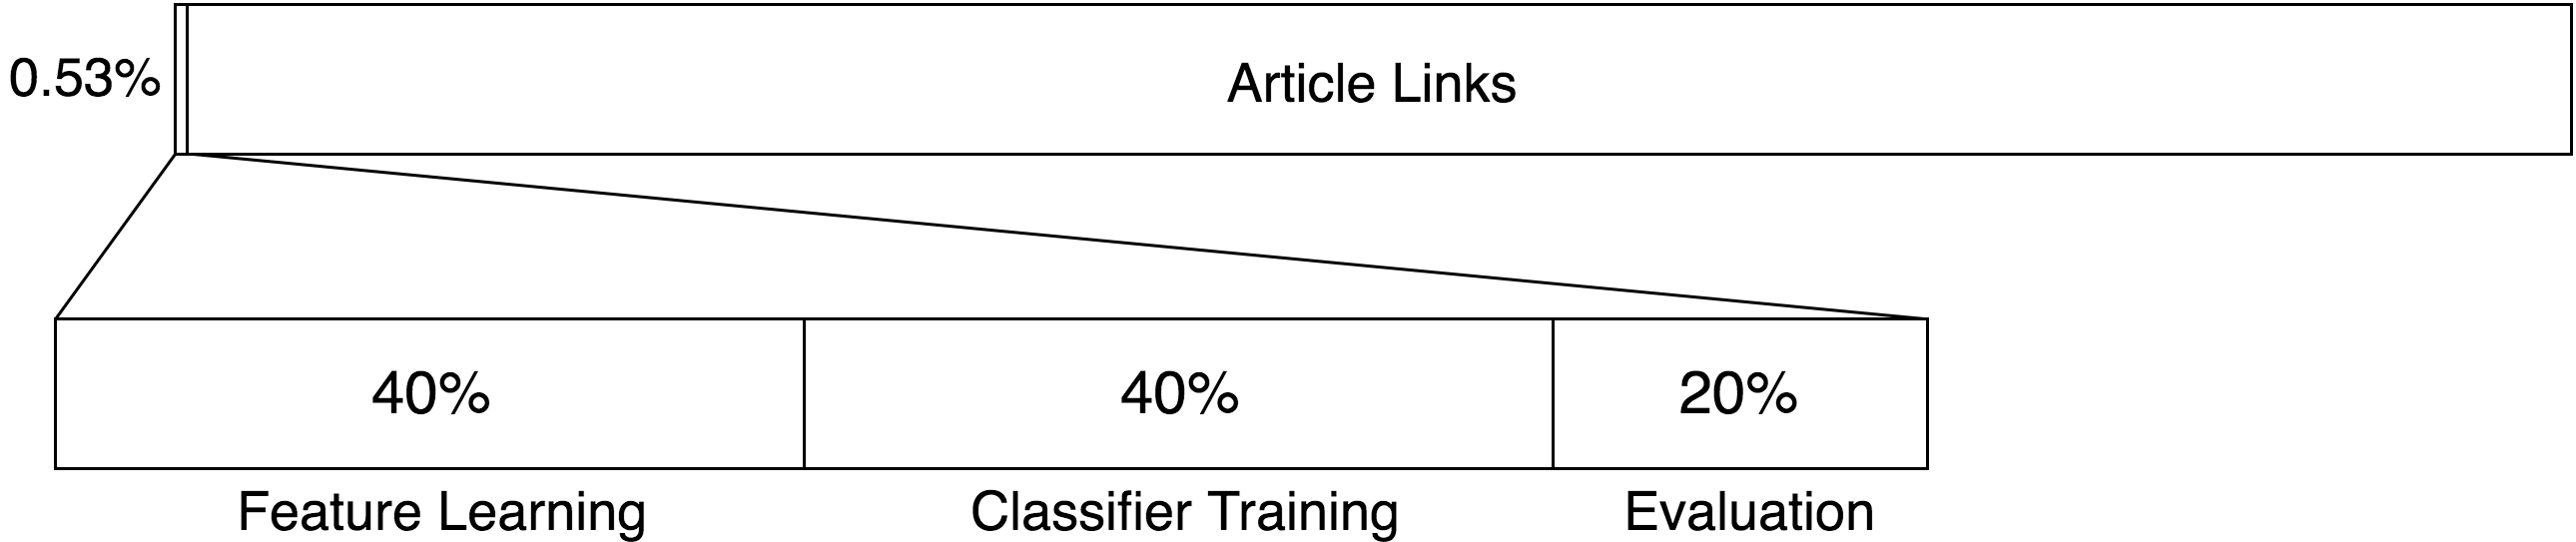
\includegraphics[width=\textwidth]{link-distribution}
\end{frame}
\note{
  \begin{itemize}
    \item Small proportion
    \item Ground truth
  \end{itemize}
}


\begin{frame}
    \centering
    \resizebox{\textwidth}{!}{%
      \begin{tikzpicture}[node distance = 2.84cm, auto]
    \node [database, yshift=1em] (db) {DB};
    \node [bigblock, right of=db] (ap) {Article Picker};
    \node [bigblock, right of=ap] (tfl) {Feature Extraction};
    \node [bigblock, right of=tfl] (classifier) {Classifier};
    \node [database, right of=classifier] (db2) {DB2};
    \node [bigblock, below=1cm of db2] (web) {Web Interface};
    
    %\node [above=1cm of ap] (inputarticle) {};
    
    \node [smallblock, below=1.5cm of ap, xshift=-2em] (n2v) {Node2Vec};
    \node [smallblock, below=.5cm of n2v] (paropt) {Parameter Optimizer};
    
    \node [smallblock, below=4.5cm of tfl] (prepper) {Training Data Generator};
    \node [smallblock, right of=prepper] (classifierTrainer) {Classifier Trainer};
    
    \begin{scope}[on background layer]
    \node [container, fit=(n2v)(paropt)] (container1) {};
    \node[below] at (container1.north) {Feature Learning};
    \node [container, fit=(prepper)(classifierTrainer)] (container2) {};
    \node[above] at (container2.south) {Classifier Model Learning};
    
    \node [container, fit=(db)(db2)] (container3) {};
    \node[below] at (container3.north) {Main Pipeline};
    \end{scope}
    
    %\draw [->] (db) -- (n2v);
    
    \path [line] (db) -- (ap);
    %\path [line] (inputarticle) -- (ap);
    \path [line] (ap) -- (tfl);
    \path [line] (tfl) -- (classifier);
    \path [line] (classifier) -- (db2);
    \path [line] (db2) -- (web);
    
    \path [line] (db.300) |- (n2v);
    %\path [line] (db.300) |- (paropt);
    \path [line] (db.240) |- (prepper);
    
    \path [line, swap, transform canvas={xshift=-1.3em}] (paropt) -- node{Parameters} (n2v);
    \path [line] (n2v.east) -| node [near end] {Model} ([xshift=-1.2em]tfl.south);
    
    \path [line] (prepper) -- (classifierTrainer);
    %\path [line] (prepper) -- (tfl);
    %\path [line] ([xshift=1.2em]tfl.south) -- ([xshift=1.2em]prepper.north);
    \draw [line] (prepper.north) |- ([xshift=1.2em, yshift=0.5em]tfl.south) -- ([xshift=1.2em]prepper.north);
    
    \path [line] (classifierTrainer) -- node{Model} (classifier);
    
  \end{tikzpicture}
    }
\end{frame}


\begin{frame}
    \frametitle{Feature Learning}
    %\framesubtitle{Data Partitioning}
    \centering

    \begin{itemize}
      \item node2vec
      \item Article features
    \end{itemize}

    
\includegraphics[width=\textwidth]{feature-learning}
\end{frame}
\note{
  \begin{itemize}
    \item Notes here...
  \end{itemize}
}


\begin{frame}
    \frametitle{Feature Extraction}
    %\framesubtitle{Data Partitioning}
    \centering

    \begin{itemize}
      \item Combine article features
      \item non-commutative operation
    \end{itemize}

   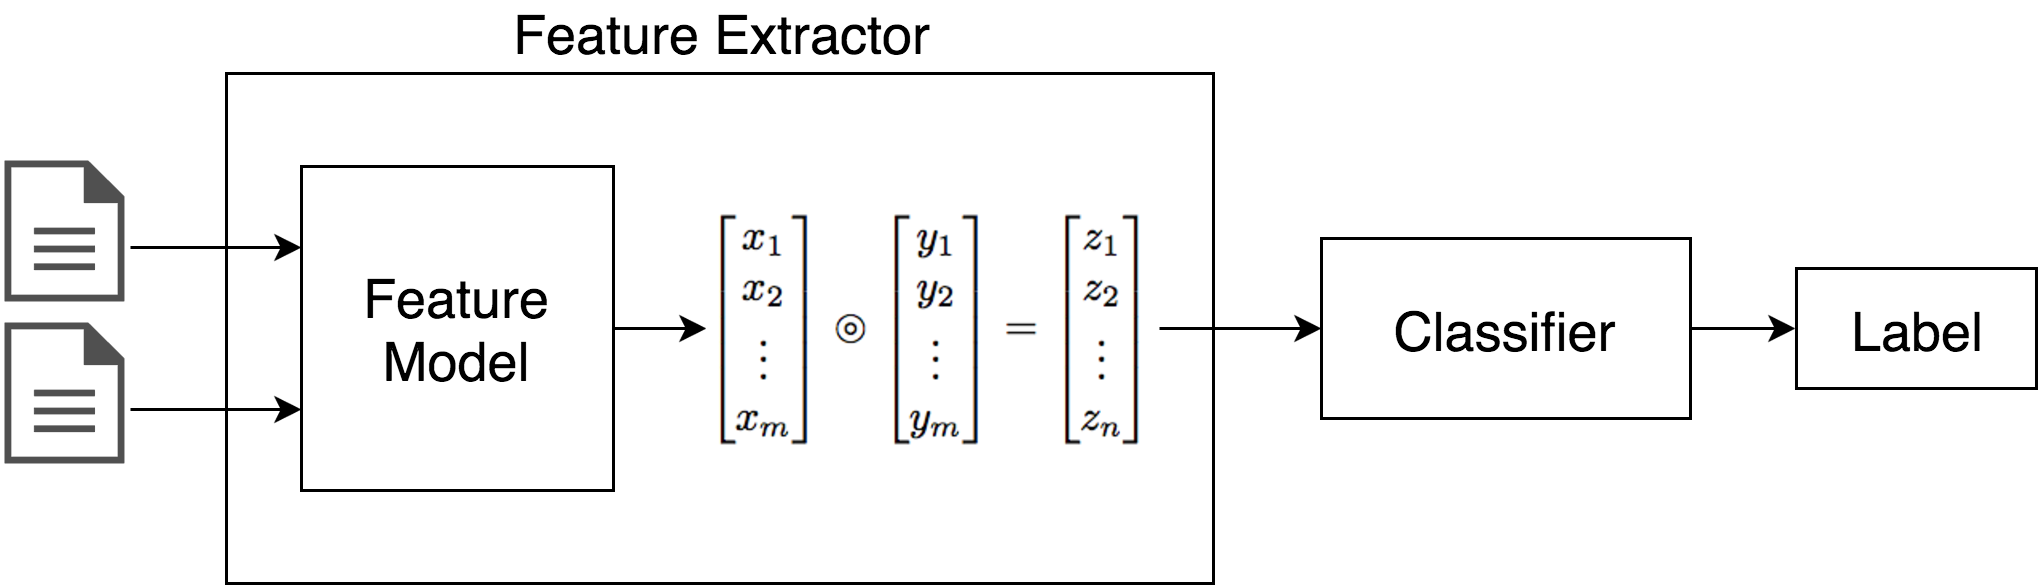
\includegraphics[width=\textwidth]{feature-extractor}
\end{frame}
\note{
  \begin{itemize}
    \item Concatenation
  \end{itemize}
}


\begin{frame}
    \frametitle{Classification}
    %\framesubtitle{Data Partitioning}
    \centering

    \begin{itemize}
      \item 10-fold cross-validation
    \end{itemize}

    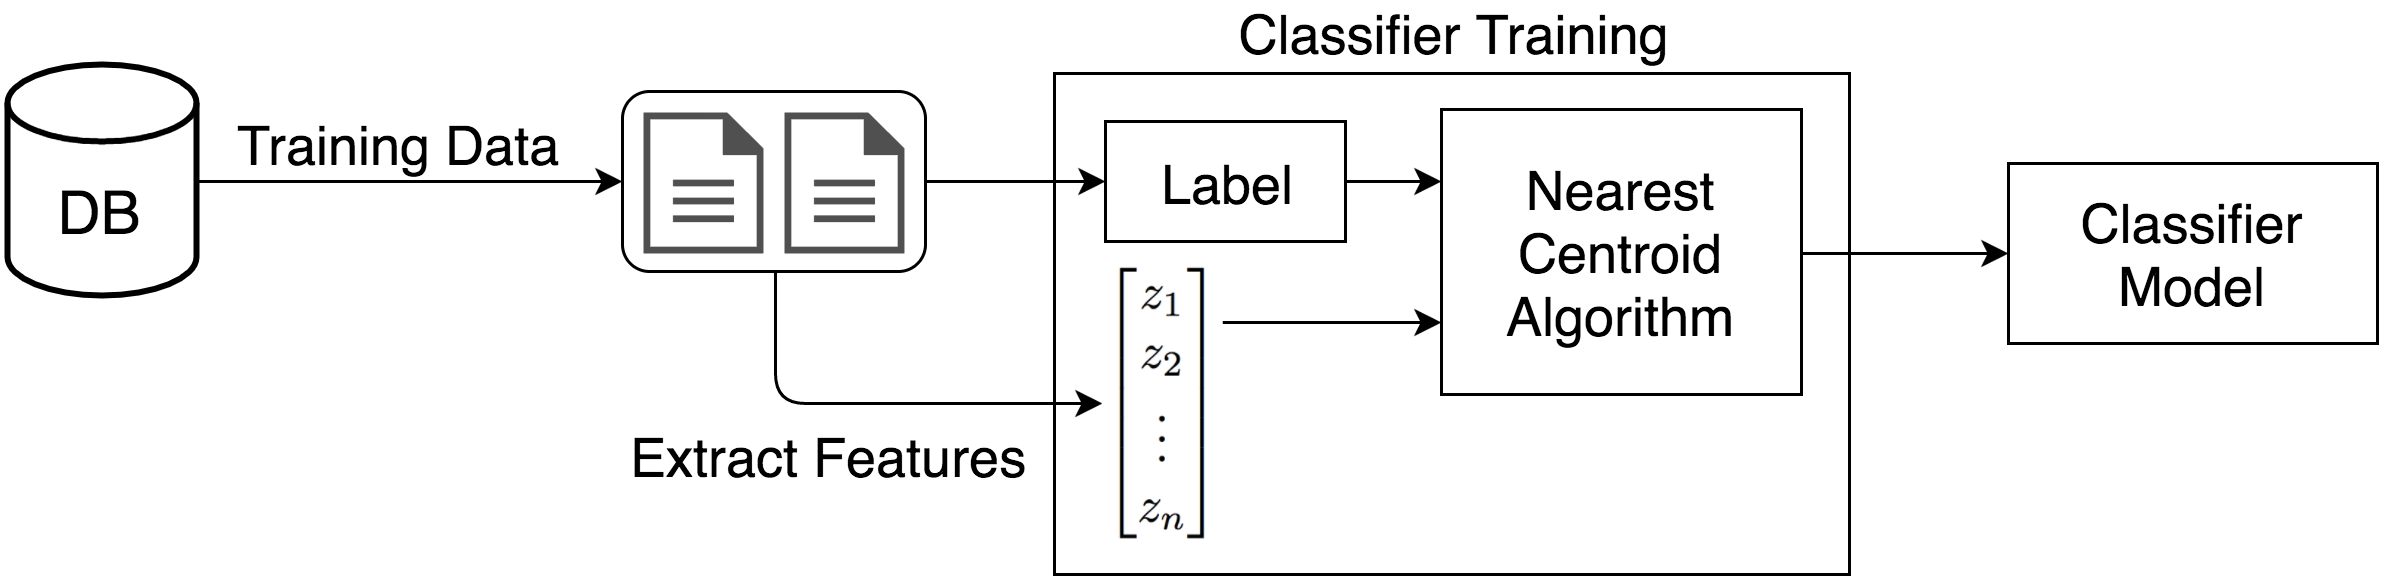
\includegraphics[width=\textwidth]{classifier-training}
\end{frame}
\note{
  \begin{itemize}
    \item Positive/Negative training samples
  \end{itemize}
}


\begin{frame}
    \frametitle{Machine Learning Pipeline}
    \framesubtitle{Components}
    \centering

    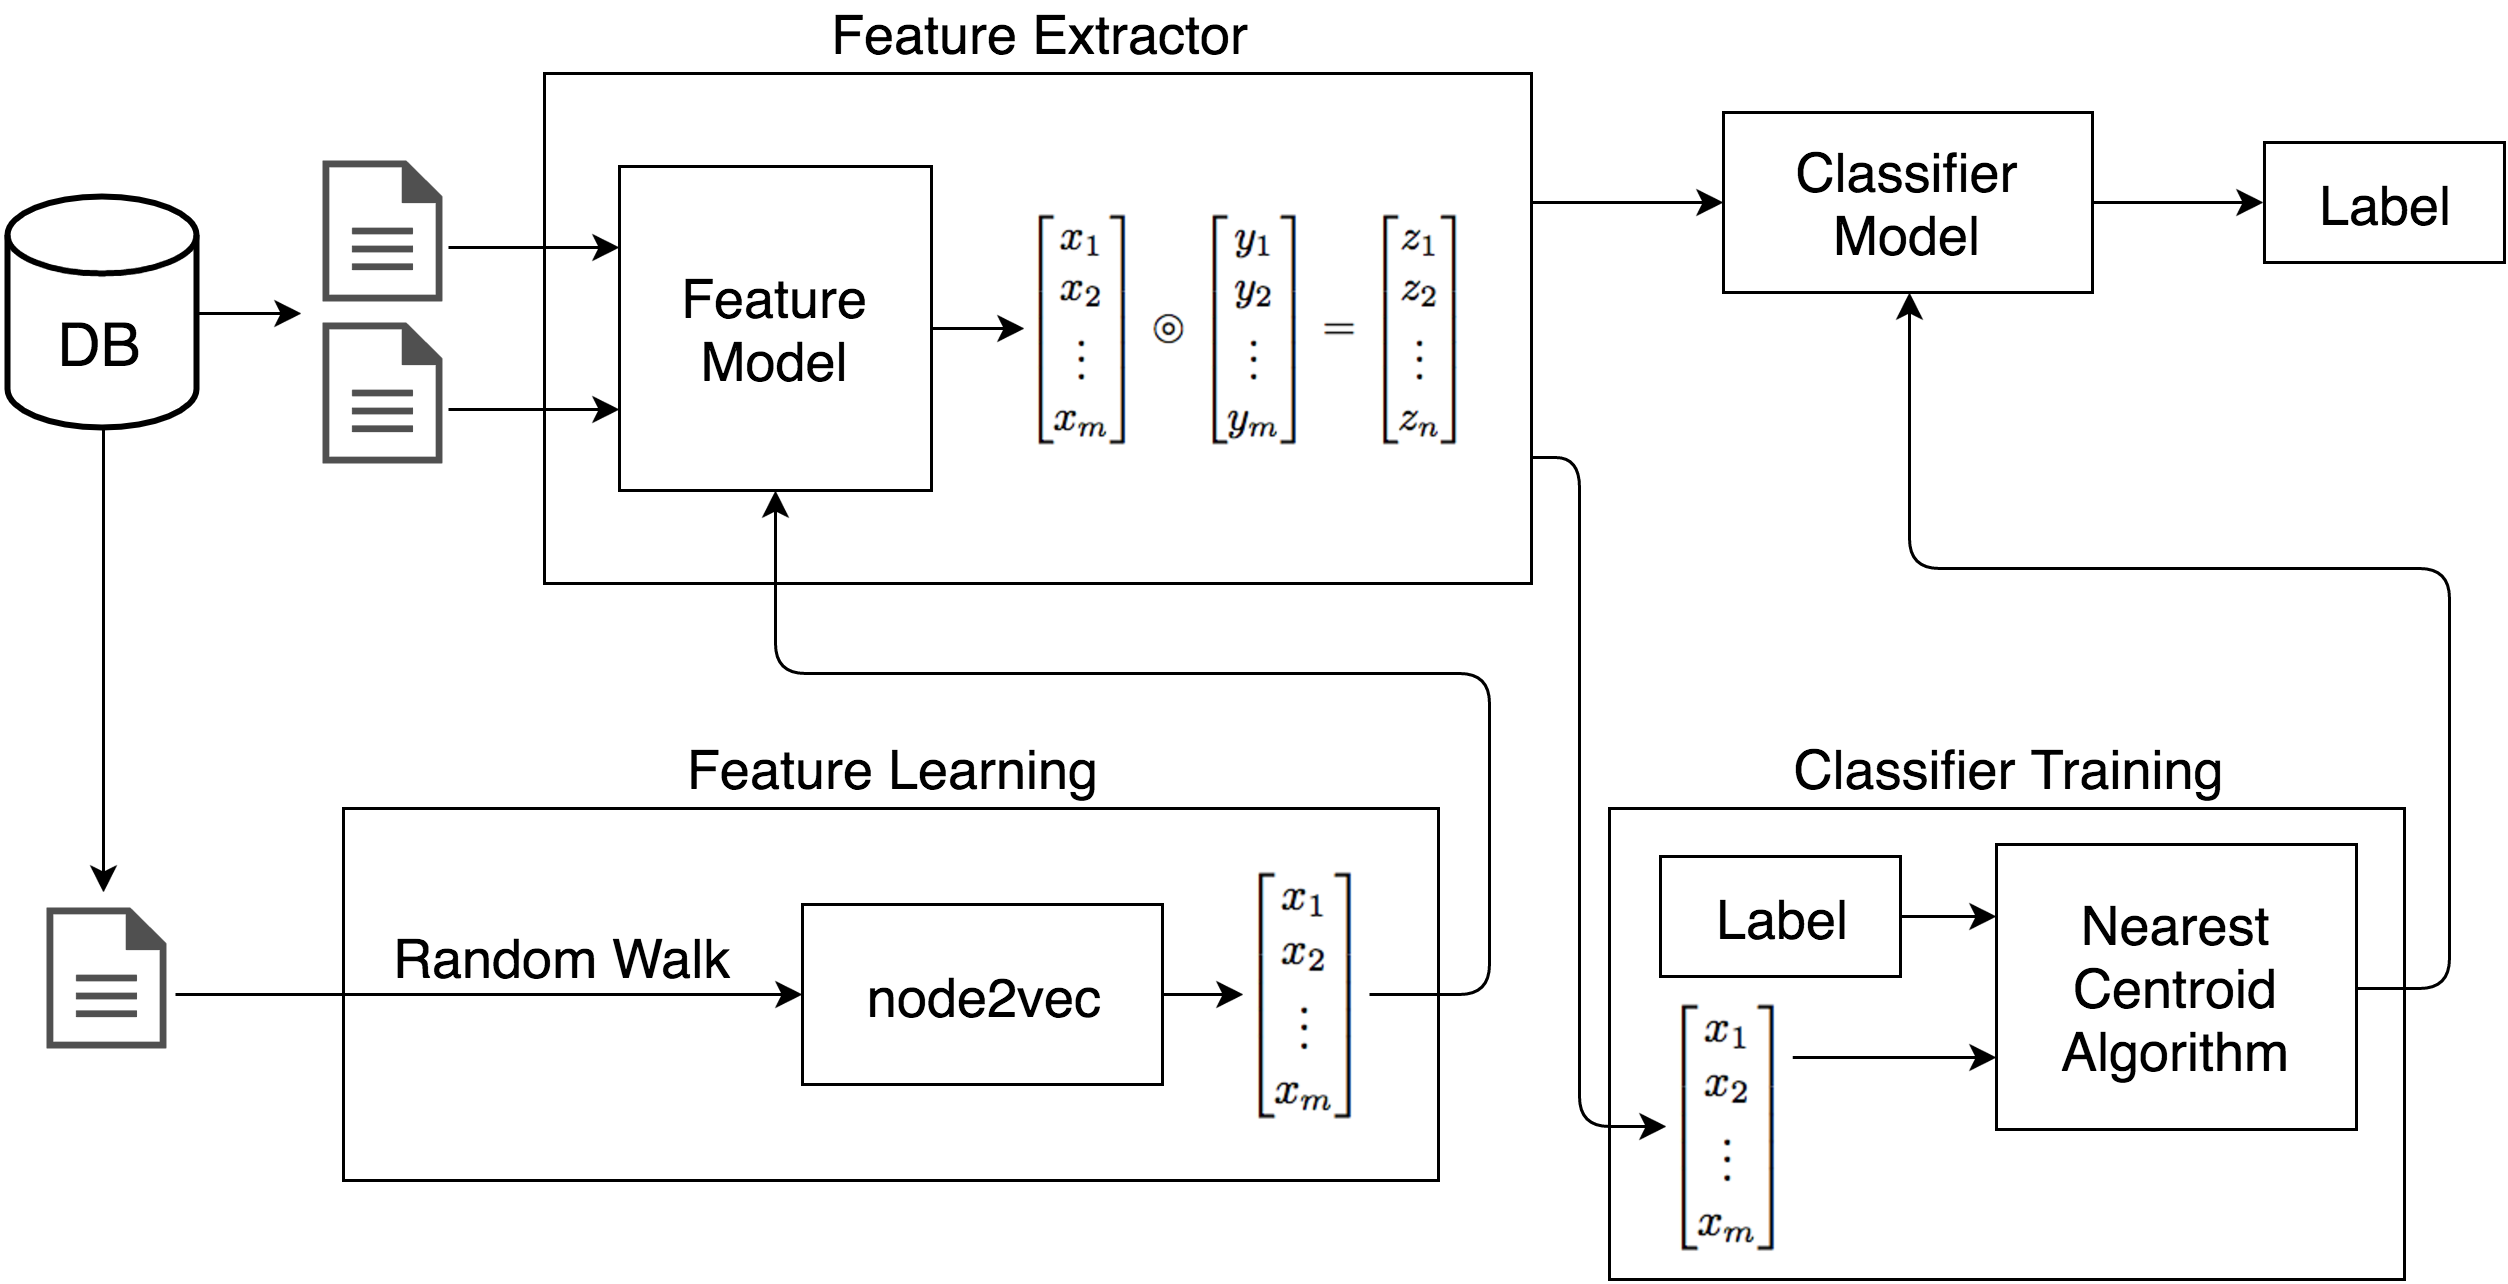
\includegraphics[width=\textwidth]{pipeline}
\end{frame}


\begin{frame}
    \frametitle{Machine Learning Pipeline}
    \framesubtitle{Components}
    \centering

    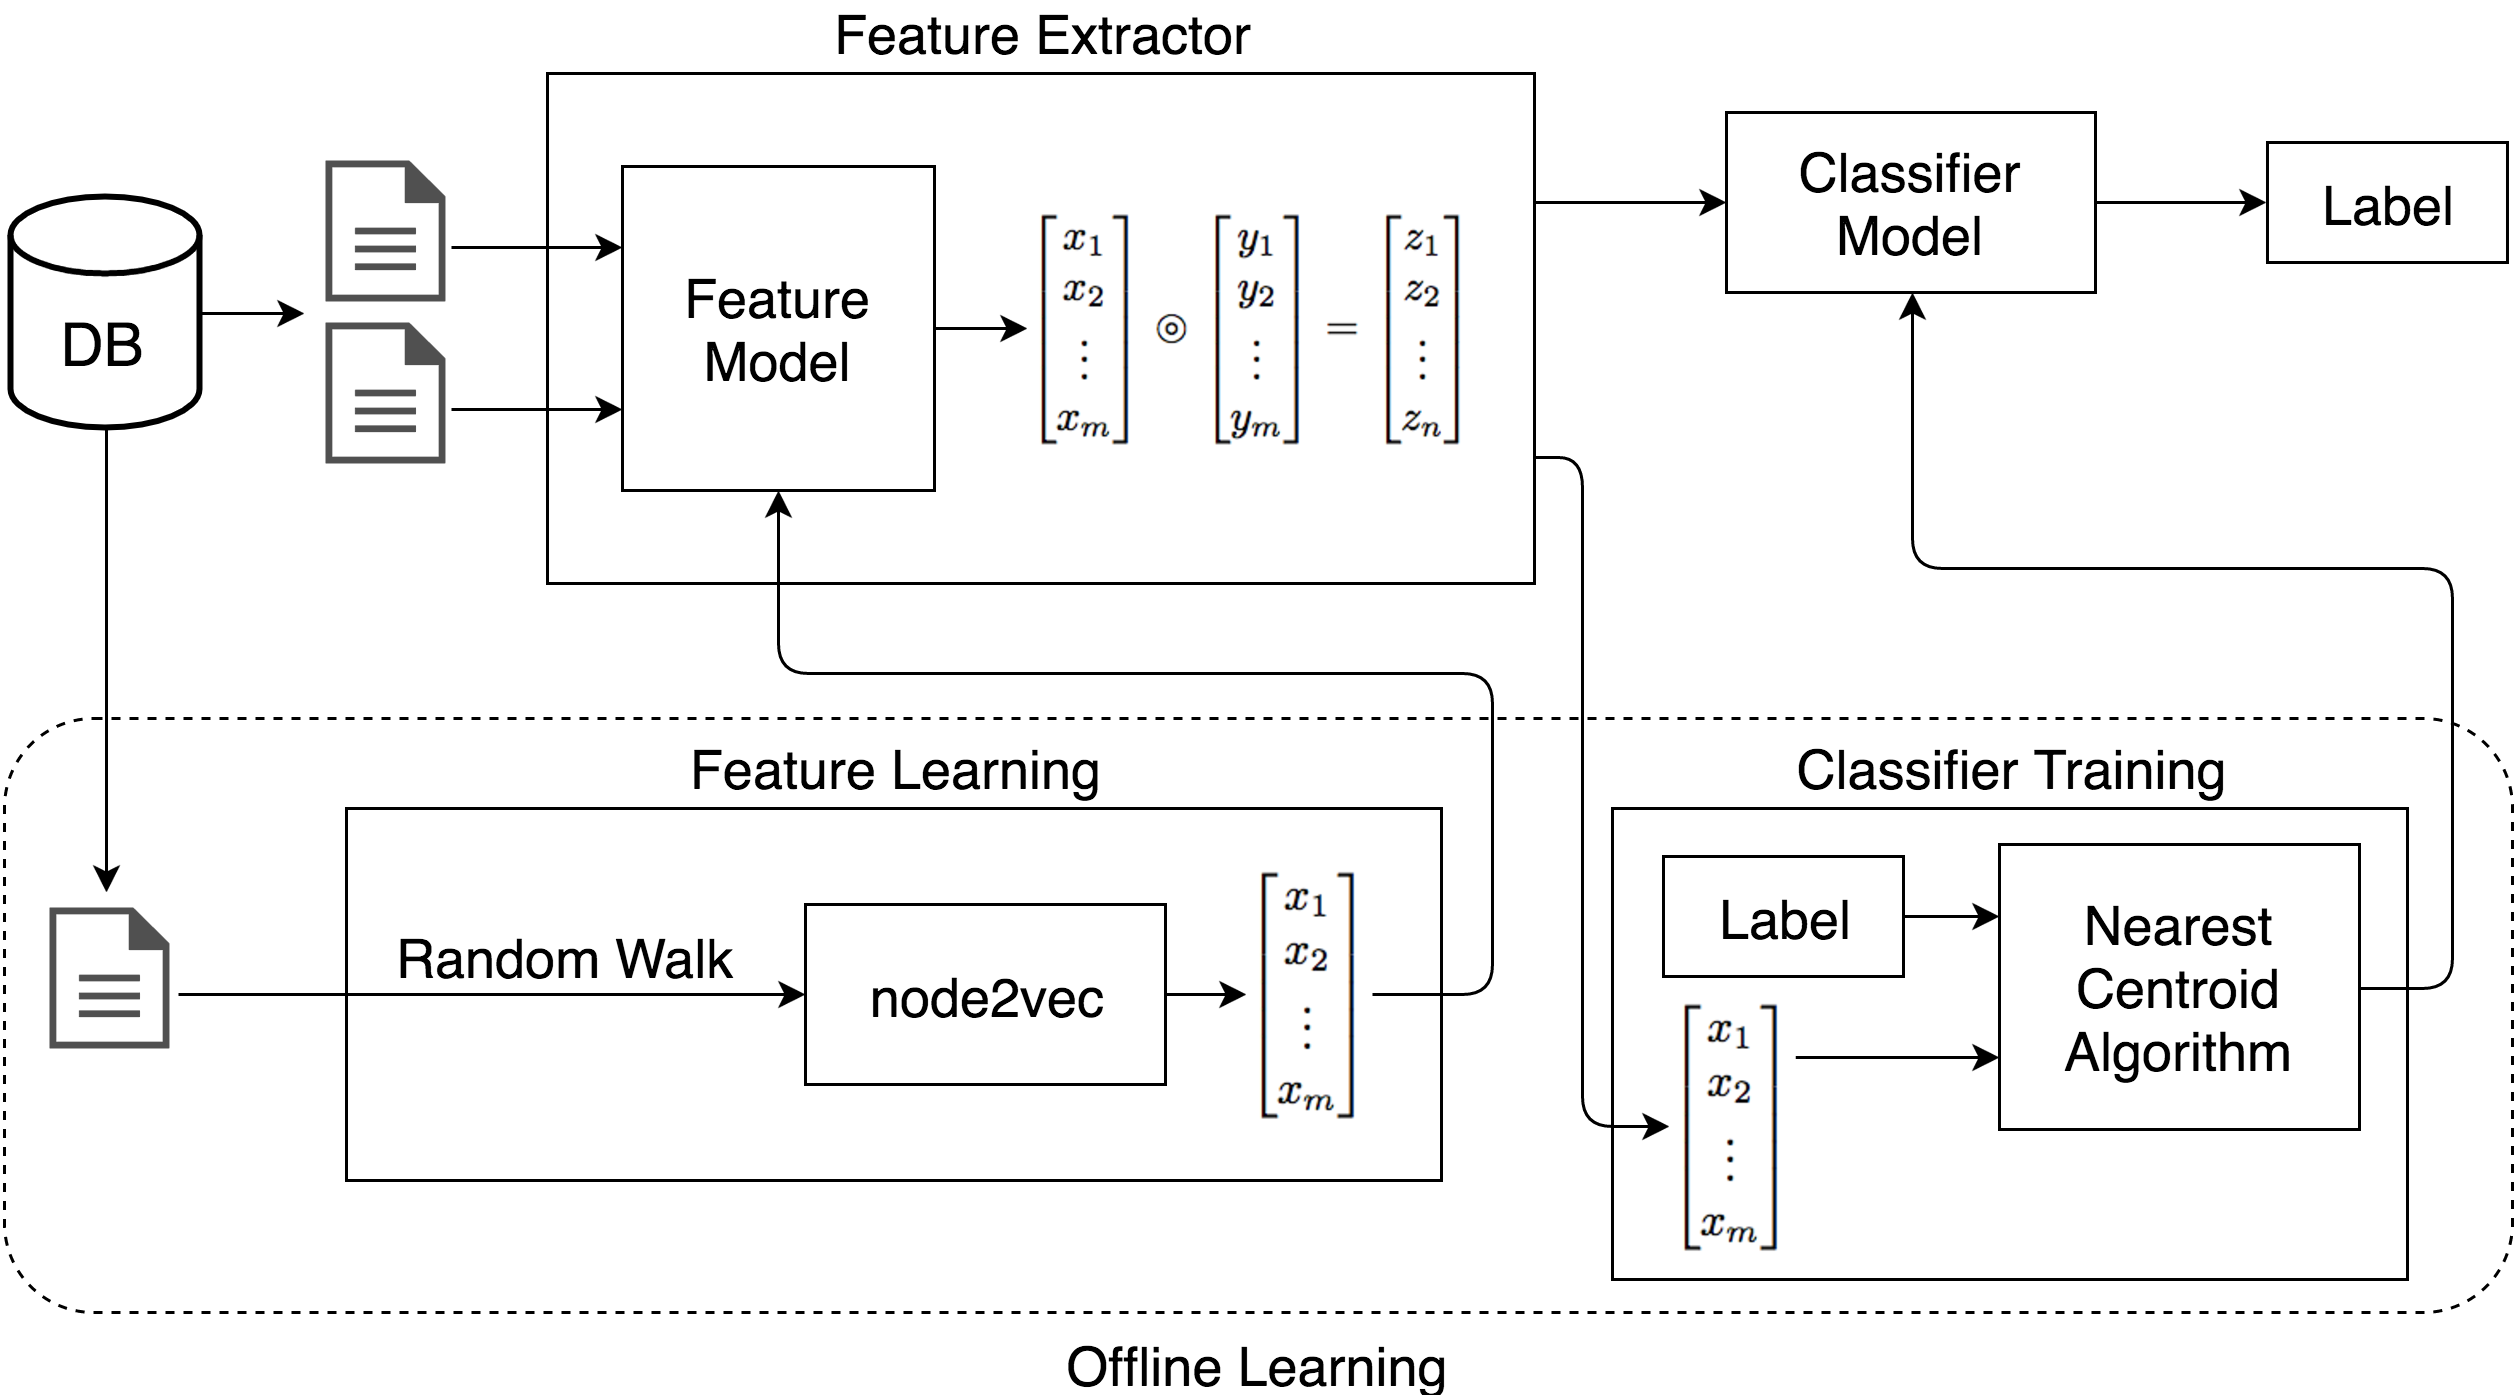
\includegraphics[width=\textwidth]{pipeline2}
\end{frame}
\note{
  \begin{itemize}
    \item Online/Offline Learning
  \end{itemize}
}
